\documentclass{article}
\usepackage[preprint]{neurips_2026}
\usepackage[utf8]{inputenc}
\usepackage[T1]{fontenc}
\usepackage{amsmath,amssymb}
\usepackage{booktabs}
\usepackage{graphicx}
\usepackage{url}
\makeatletter
\renewcommand{\@noticestring}{ES 678 Course Project --- IIT Gandhinagar}
\makeatother

\title{Feature-Based Inventory Demand Forecasting on M5 Walmart Data: What History, Calendar, and Price Add}
\author{Arpit Metrey \\ Roll Number: 26210175 \\ Indian Institute of Technology Gandhinagar \\ \texttt{arpit.metrey@iitgn.ac.in}}

\begin{document}
\maketitle

\begin{abstract}
We measure how much historical sales, calendar events, and selling price add to 28-day-ahead daily retail demand forecasts over simple baselines. Using a stratified subset of 1,000 item--store series (1.5M item--store--days) from the M5 Walmart dataset, we compare Ridge regression and gradient-boosted decision trees under chronological train/validation/test splits, feature-group ablations, and paired bootstrap tests over series. Both models beat the strongest benchmark, a four-week same-weekday mean, by 3.6\% in MAE and 8\% in RMSE on the held-out test horizon, with bootstrap confidence intervals excluding zero; Ridge and boosted trees are statistically indistinguishable. Lagged sales history accounts for over 90\% of the MAE reduction of the full models, calendar variables add modest gains, and price adds negligible lift once history is present. Learned models underperform simple baselines on zero-sales days and slow-moving items because of loss-metric misalignment under intermittent demand.
\end{abstract}

\section{Problem and Motivation}
Retailers must set replenishment quantities weeks before demand occurs, so a key question is how accurately daily unit sales can be predicted four weeks ahead and which data features give real predictive lift. We investigate this problem using the M5 Walmart dataset \citep{makridakis2022}. Each record represents an item--store--day observation, where target $y_{i,t}$ denotes unit sales for series $i$ (one item within a specific store) on day $t$. Forecasts are generated at origin day $T$ for the 28-day target horizon $t=T+1,\dots,T+28$, utilizing historical observations up to $T$ alongside deterministic forward variables (calendar events and planned prices).

Our core research inquiry examines: \emph{To what extent do historical sales, calendar information, and price features improve 28-day retail demand forecasts over baseline heuristics?} The results describe predictive performance on this horizon and series subset only; they do not support causal claims such as price elasticity.

\section{Data and Preparation}
\textbf{Source and sample.} We utilize the Kaggle M5 Forecasting data, encompassing daily sales for 30,490 item--store series across 10 stores (California, Texas, Wisconsin) over 1,941 days, supplemented by calendar attributes (holidays, SNAP food-assistance schedules) and weekly selling prices. For efficiency, we sample 1,000 series (100 per store) maintaining category proportions matching the parent dataset (47\% FOODS, 19\% HOBBIES, 34\% HOUSEHOLD). Stratification was performed strictly on metadata using random seed 42, independently of sales volume.

\textbf{Quality checks.} Sales quantities contain no negative entries; 68\% of total raw observations are zero. Every series exhibits consecutive leading zeros prior to its initial price entry, corresponding to pre-launch availability. Dropping these 21.4\% pre-launch rows leaves 1,525,319 active observations (58.8\% zeros, mean 1.57 units/day, maximum 166). Retained records contain no missing price values. The validation and evaluation files agree on all shared days. Missing event names initially loaded as empty strings rather than nulls, creating constant indicator features; this was fixed before the final runs.

\textbf{Preprocessing.} All historical features are constructed using sales lags of at least 28 days ($s \le t-28$), preventing temporal leakage across the forecast horizon. Feature standardization parameters (means and variances for Ridge regression) were computed exclusively from training rows ($d \le 1885$). Volume tiers use the final 91 training days ($d\in[1795,1885]$). All model outputs are non-negatively clipped at zero.

\section{Methods}
\textbf{Baselines.} Defining horizon $h=t-T$ and $k=\lceil h/7\rceil$:
\begin{enumerate}\setlength{\itemsep}{0pt}\setlength{\parsep}{0pt}
\item \emph{Zero forecast:} $\hat y=0$.
\item \emph{Seasonal naive} \citep{hyndman2021}: same-weekday sales from the most recent pre-origin week, $\hat y_{i,t}=y_{i,t-7k}$.
\item \emph{Four-week weekday mean:} average sales on the same weekday over the prior four weeks, $\hat y_{i,t}=\frac14\sum_{j=0}^{3}y_{i,t-7(k+j)}$. This serves as our primary reference benchmark.
\end{enumerate}

\textbf{Direct 28-day formulation.} We train single multi-horizon models on rows $(i,t)$ constrained to features derived from $y_{i,s}$ where $s\le t-28$. This direct formulation estimates demand across the entire 28-day window without recursive auto-regression. Features are structured into four primary blocks:
\begin{itemize}\setlength{\itemsep}{0pt}\setlength{\parsep}{0pt}
\item \emph{History:} lags $y_{i,t-\ell}$ for $\ell\in\{28,35,42,56\}$, plus 7-day and 28-day rolling averages ending at $t-28$.
\item \emph{Calendar:} day-of-week, month, event type, and state-level SNAP assistance indicators.
\item \emph{Price:} selling price and price ratio relative to 28 days prior ($P_t/P_{t-28}$).
\item \emph{Static:} store and category one-hot encodings.
\end{itemize}

\textbf{Learned models.} Ridge regression \citep{hoerl1970} minimizes $\sum_{(i,t)}(y_{i,t}-w^\top x_{i,t}-b)^2+\alpha\lVert w\rVert_2^2$ over $(w,b)$ on standardized inputs. Gradient-boosted decision trees \citep{friedman2001} (\texttt{HistGradientBoostingRegressor} \citep{pedregosa2011}) ensemble 120 trees (maximum 31 leaves, learning rate 0.1, min samples leaf 200, L2 regularization 1.0) to capture nonlinear interactions (e.g., weekday $\times$ base volume).

\section{Evaluation Design}
\textbf{Split.} Experiments follow a strict chronological split: training on days $d\le1885$, validation on $1886\le d\le1913$, and testing on $1914\le d\le1941$ (2016-04-25 to 2016-05-22). Each of the validation and test periods scores 28,000 series-day cells.

\textbf{Tuning.} Ridge penalty $\alpha\in\{0.1,1,10,100,1000\}$ and GBT loss functions (squared error vs.\ Poisson deviance) were optimized on validation RMSE using models trained on $d\le1885$. Selected configurations were refit on combined data ($d\le1913$) and evaluated once on test data.

\textbf{Metrics.} Model accuracy is evaluated via Mean Absolute Error ($\mathrm{MAE}=\frac1N\sum|\hat y-y|$) and Root Mean Squared Error ($\mathrm{RMSE}=\sqrt{\frac1N\sum(\hat y-y)^2}$). Statistical significance is established using paired bootstrap sampling \citep{efron1979} across series (2,000 iterations, seed 42).

\begin{table*}[t]
\caption{Validation and test performance (units/day) across 1,000 series on the 28-day forecast horizon.}
\label{tab:main}
\centering
\begin{tabular}{lcccc}
\toprule
 & \multicolumn{2}{c}{Validation} & \multicolumn{2}{c}{Test} \\
Method & MAE & RMSE & MAE & RMSE \\
\midrule
Zero forecast & 1.604 & 3.877 & 1.556 & 3.539 \\
Seasonal naive & 1.357 & 2.835 & 1.292 & 2.466 \\
4-week weekday mean & 1.137 & 2.162 & 1.157 & 2.130 \\
Ridge (all features) & 1.114 & 2.109 & 1.115 & 1.966 \\
Boosted trees (all features) & \textbf{1.106} & \textbf{2.062} & \textbf{1.114} & \textbf{1.948} \\
\bottomrule
\end{tabular}
\end{table*}

\begin{figure*}[t]
\centering
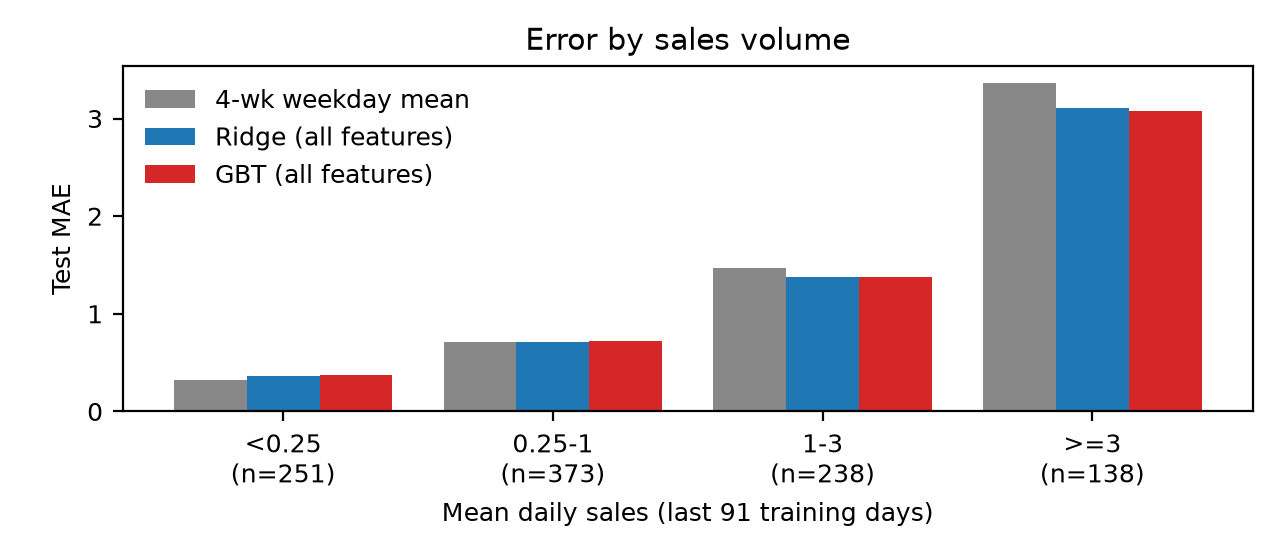
\includegraphics[width=0.7\textwidth]{results/figures/fig3_volume.png}
\caption{Test MAE by daily sales volume tier (mean daily sales over the last 91 training days). Models gain on high-volume items but underperform simple baselines on low-volume series.}
\label{fig:volume}
\end{figure*}

\section{Results and Error Analysis}
Table~\ref{tab:main} summarizes benchmark results. Both machine learning models outperform the 4-week weekday baseline on test data: Ridge reduces MAE from 1.157 to 1.115 (3.6\% improvement) and RMSE from 2.130 to 1.966 (7.7\% improvement). Boosted trees achieve 1.114 MAE (3.7\% improvement) and 1.948 RMSE (8.5\% improvement). Paired bootstrap testing confirms statistical significance against the baseline: MAE differences are $-0.041$ for Ridge (95\% CI $[-0.058,-0.025]$) and $-0.042$ for GBT (95\% CI $[-0.064,-0.021]$). GBT and Ridge performance is statistically equivalent (MAE difference $-0.001$, 95\% CI $[-0.011,0.008]$).

\textbf{Error breakdown.} Error rates remain constant across the 28-day horizon (weekly block MAE for GBT: 1.06, 1.15, 1.14, 1.10), reflecting the fixed direct lag structure ($\ell\ge28$). GBT outperforms the baseline across all product categories (FOODS MAE 1.440 vs.\ 1.491) and in 9 of 10 individual stores (Ridge: 10 of 10 stores).

\textbf{Failure modes.} Performance varies substantially across sales volume tiers (Figure~\ref{fig:volume}). Fast-selling series ($\ge3$ units/day, representing 55\% of total volume across 138 series) show clear model gains (GBT MAE 3.08 vs.\ 3.36 baseline). Conversely, on low-volume series ($<0.25$ units/day, $n=251$), the weekday baseline achieves lower MAE (0.318 vs.\ 0.377 GBT). On positive sales days, GBT achieves superior MAE (1.663 vs.\ 1.827 baseline), but performs worse on zero-sales days (0.622 vs.\ 0.555 baseline).

\section{Graduate Depth Analysis}
\textbf{Feature-group ablation.} Table~\ref{tab:abl} details the sequential impact of feature groups added to static store/category encodings. Historical sales lags dominate predictive accuracy: without them, every configuration except boosted trees with price only has test MAE of 1.73--1.77, worse than the zero forecast (1.556). Price alone helps boosted trees (MAE 1.413), probably because price acts as an item-identity proxy, but this gain vanishes once history is present. Calendar features provide minor secondary gains when combined with history ($\Delta$MAE $=-0.027$ Ridge, $-0.023$ GBT). Price features provide negligible incremental value once history is present ($\Delta$MAE $=-0.002$ Ridge, $-0.003$ GBT).

\begin{table*}[t]
\caption{Feature-group ablation results (Test MAE / RMSE). Static encodings are included in all models.}
\label{tab:abl}
\centering
\begin{tabular}{lcccc}
\toprule
 & \multicolumn{2}{c}{Ridge} & \multicolumn{2}{c}{Boosted trees} \\
Added groups & MAE & RMSE & MAE & RMSE \\
\midrule
None (static only) & 1.771 & 3.097 & 1.766 & 3.091 \\
+ History & 1.144 & 1.975 & 1.136 & 1.981 \\
+ Calendar & 1.743 & 3.090 & 1.732 & 3.080 \\
+ Price & 1.741 & 3.045 & 1.413 & 2.434 \\
+ History + Calendar & 1.117 & 1.967 & 1.113 & 1.959 \\
+ History + Price & 1.142 & 1.974 & 1.132 & 1.980 \\
All features & 1.115 & 1.966 & 1.114 & 1.948 \\
\bottomrule
\end{tabular}
\end{table*}

\textbf{Zero-inflation and loss-metric mismatch.} Standard regression objectives (squared error, Poisson deviance) estimate conditional means, whereas MAE is minimized by conditional medians. For highly intermittent series the median is zero, so mean-calibrated models predict small fractional units on zero-demand days and pay a consistent MAE penalty relative to sparse baselines. Overall bias stays small ($+0.002$ Ridge, $+0.006$ GBT vs.\ $+0.048$ baseline): mean calibration is preserved at the expense of zero-day MAE.

\section{Limitations and Conclusion}
\textbf{Limitations.} Evaluation uses a single 28-day window (spring 2016) and 1,000 series. Bootstrap resampling addresses series-level variance, but robustness across years and seasons needs rolling-origin evaluation.

\textbf{Conclusion.} Historical sales lags provide the primary signal for 28-day retail demand forecasting. Ridge regression and gradient-boosted trees achieve comparable accuracy improvements over standard baselines, driven primarily by gains on high-volume series.

\section{Reproducibility}
\url{https://github.com/arpitmetrey/m5-demand-forecasting} holds the code and a README with the run order. All preprocessing, feature construction, tuning, and evaluation are automated by Python scripts. Evaluation uses one chronological split, not cross-validation. Environment: Python 3.12, scikit-learn 1.9.1, pandas 3.1.0, NumPy 2.5.4, seed 42.

\textbf{AI-use disclosure.} The topic, research question, and proposal are my own. Claude (Anthropic) helped with design suggestions, writing and debugging scripts, flagging output problems, and drafting text; I ran every script locally.

\begin{thebibliography}{6}
\bibitem[Makridakis et~al.(2022)]{makridakis2022} S.~Makridakis, E.~Spiliotis, and V.~Assimakopoulos. M5 accuracy competition: Results, findings, and conclusions. \emph{International Journal of Forecasting}, 38(4):1346--1364, 2022.
\bibitem[Hyndman and Athanasopoulos(2021)]{hyndman2021} R.~J. Hyndman and G.~Athanasopoulos. \emph{Forecasting: Principles and Practice}, 3rd ed. OTexts, 2021.
\bibitem[Hoerl and Kennard(1970)]{hoerl1970} A.~E. Hoerl and R.~W. Kennard. Ridge regression: Biased estimation for nonorthogonal problems. \emph{Technometrics}, 12(1):55--67, 1970.
\bibitem[Friedman(2001)]{friedman2001} J.~H. Friedman. Greedy function approximation: A gradient boosting machine. \emph{Annals of Statistics}, 29(5):1189--1232, 2001.
\bibitem[Pedregosa et~al.(2011)]{pedregosa2011} F.~Pedregosa et~al. Scikit-learn: Machine learning in Python. \emph{Journal of Machine Learning Research}, 12:2825--2830, 2011.
\bibitem[Efron(1979)]{efron1979} B.~Efron. Bootstrap methods: Another look at the jackknife. \emph{Annals of Statistics}, 7(1):1--26, 1979.
\end{thebibliography}
\end{document}
